	จากการค้นคว้าหาเครื่องมือในการ labeling เพื่อใช้เป็นแนวทางในการทำ Goggle labeling tool พบเครื่องมือที่เป็น open source เปิดให้ทดลองใช้อยู่ 2 เครื่องมือ คือ DarkLabel และ OpenLabeling โดยสรุปข้อสำคัญได้ดังนี้ 

\subsubsection*{โปรแกรม DarkLabel}
เป็นโปรแกรมที่ช่วยในการทำนายคำอธิบายและบันทึกในรูปแบบต่างๆ รองรับข้อมูลอินพุทในรูปแบบไฟล์วิดีโอ avi , mpg หรือ กลุ่มรูปภาพ มีขั้นตอนการ labeling ดังนี้ 
\begin{enumerate}
	\setlength\itemsep{-0.25em}
	\item สร้างกรอบสี่เหลี่ยม(boundary box)ครอบบริเวณวัตถุที่สนใจ โดยใช้มนุษย์เป็นคนสร้าง
	\item กดปุ่ม Next และ Predict อย่างต่อเนื่อง เพื่อ track กรอบสี่เหลี่ยม ในเฟรมถัดๆไป จนกระทั่งการ track เกิดพลาดไป
	\item ลบกรอบสี่เหลี่ยมที่พลาด และเริ่มทำขั้นตอนที่ 1 ใหม่ อีกครั้งจนครบทุกเฟรมในวิดีโอ
\end{enumerate}
หลังจากที่ผู้วิจัยได้ทดลองใช้โปรแกรม DarkLabel พบว่า เป็นโปรแกรมที่ค่อนข้างมีการทำงานส่วนใหญ่ที่เป็นการสร้างคำอธิบายแบบใช้มนุษย์เป็นคนกำหนดเองเป็นส่วนใหญ่ ซึ่งทำให้ใช้เวลาในการทำนาน และ เสียพลังงานในการทำเป็นอย่างมาก 


\begin{figure}[!ht]
	\centering
	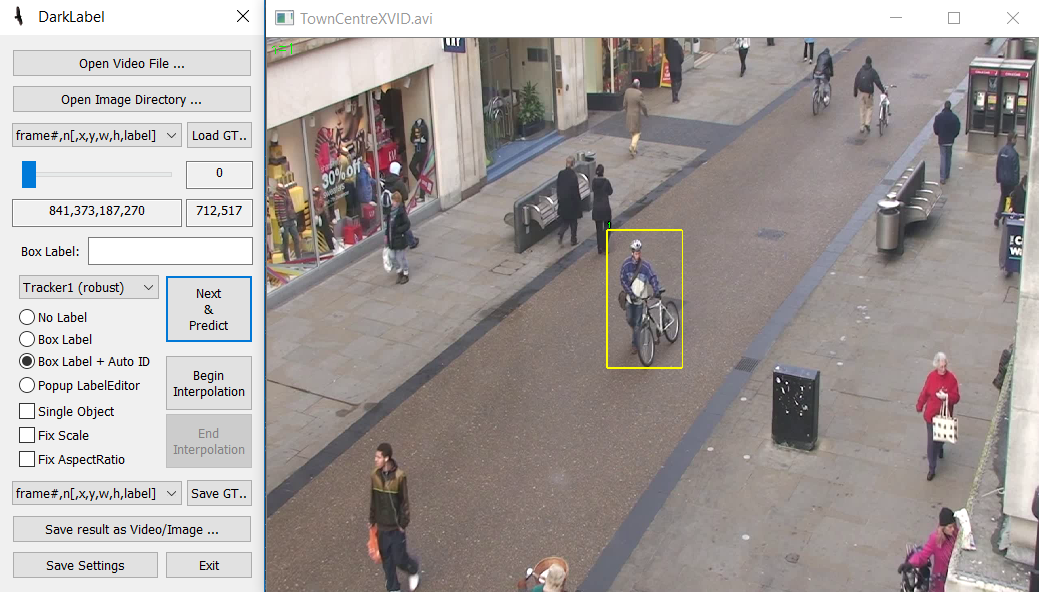
\includegraphics[width=0.7\textwidth]{chapter2/images/darklabel.png}
		\caption{UI ของโปรแกรม DarkLabel}
    	\label{fig:darklabel}
\end{figure}


\clearpage
\subsubsection*{โปรแกรม OpenLabeling}
ที่ช่วยในการทำนายคำอธิบาย โดยโปรแกรมจะมีการทำงานอยู่ 2 โหมดการทำงาน คือ แบบทำด้วยมือ และ แบบอัตโนมัติ ซึ่งมีการทำงานแยกจากกันอย่างชัดเจน 

\begin{enumerate}
	\setlength\itemsep{-0.25em}
	\item Mode Auto
	\\ หลังจากอินพุตวิดีโอเข้าไปในโปรแกรมแล้วมีขั้นตอนการ labeling ดังนี้ 
   	\begin{enumerate}
	\setlength\itemsep{-0.25em}
    		\item โปรแกรมจะทำงานอัตโนมัติ โดยใช้โมเดลในการทำนายคีย์เฟรม (predict keyframe)  และ track ในภาพที่เหลือ ผลลัพธ์ที่ได้คือ ข้อมูลของชุดข้อมูล
 	\end{enumerate}
	\item Mode Manual
	\\ หลังจากอินพุตวิดีโอเข้าไปในโปรแกรมแล้วมีขั้นตอนการ labeling ดังนี้ 
	\begin{enumerate}
	\setlength\itemsep{-0.25em}
    		\item สร้างกรอบสี่เหลี่ยม (bounding box) ขึ้นมาโดยใช้มนุษย์เป็นคนสร้าง
		\item กดปุ่มเพื่อแทร็กกรอบสี่เหลี่ยม (track bounding box) ในเฟรมถัดๆไป จนกระทั่งการแทร็กกรอบสี่เหลี่ยม (track bounding box) เกิดพลาดไป
		\item ลบกรอบสี่เหลี่ยม (bounding box) ที่พลาด และ เริ่มทำขั้นตอนที่ 1 อีกครั้งจนครบทุกเฟรมในวิดีโอ
 	\end{enumerate}
 \end{enumerate}
หลังจากที่ได้ทดลองใช้โปรแกรม OpenLabeling ทั้ง 2 โหมดการทำงานแล้วพบว่า การทำงานแบบ mode auto การที่เราไม่สามารถปรับแก้ไขสิ่งใดในระหว่างกระบวนการ labeling นั้น ทำให้หากเกิดกรณีที่โมเดลทำนายกรอบสี่เหลี่ยม (predict bounding) พลาด หรือ เกินมา เราจะไม่สามารถแก้ไขได้ และ การทำงานแบบ mode manual ไม่มีระบบตรวจสอบกรอบสี่เหลี่ยม (detect bounding box) ทำให้ผู้ใช้งานจะต้องสร้างกรอบสี่เหลี่ยม (bounding box) ขึ้นมาเอง

\begin{figure}[!ht]
	\centering
	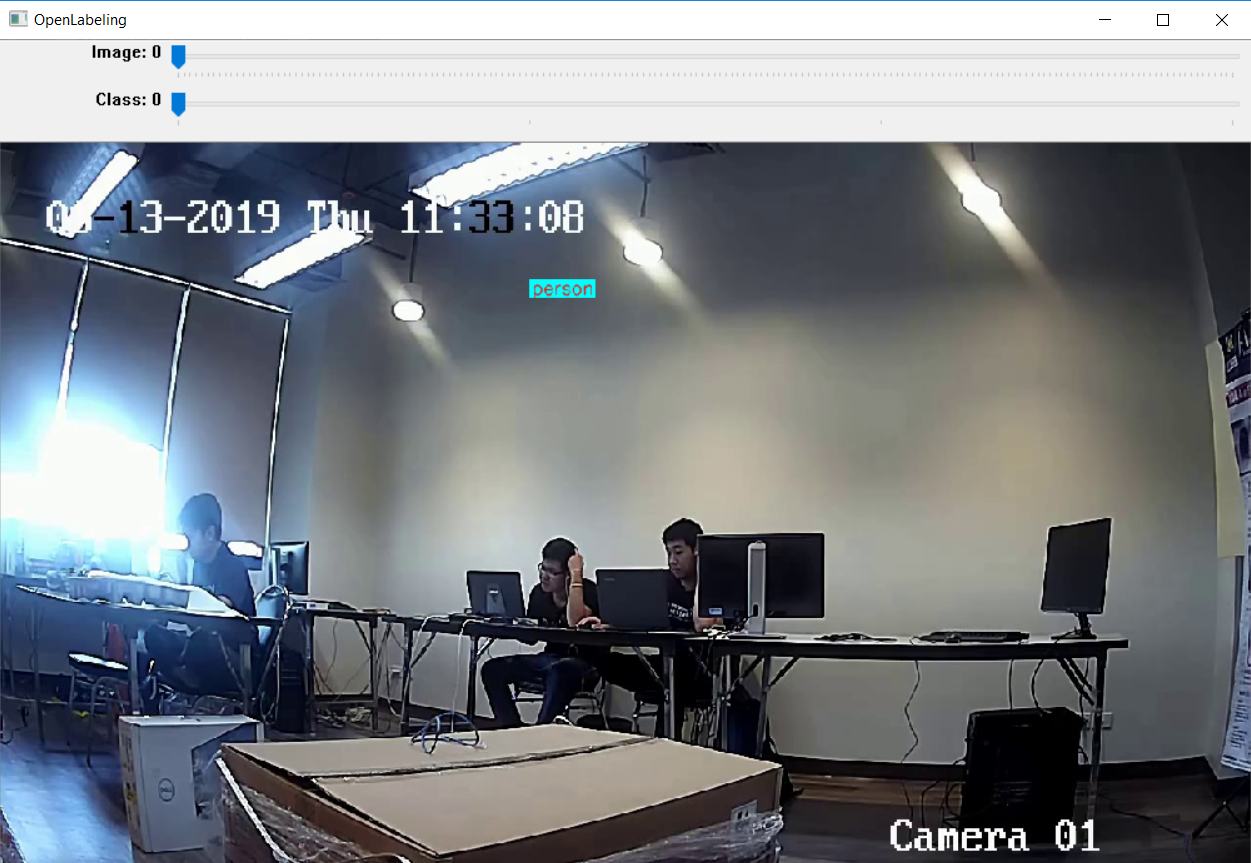
\includegraphics[width=0.7\textwidth]{chapter2/images/openlabel.png}
		\caption{UI ของโปรแกรม OpenLabeling}
    	\label{fig:openlabel}
\end{figure}


